%
%-----------------------------------------------------------
%% Computer Music Journal LaTeX template
%%
%% September  2009
%% Author: Cornelia Kreutzer, University of Limerick

% Maximum of 32 pages in the PDF including figures and references.
% Present first abstractly, then illustrate concretely, then 
% discuss examples. 
% Include figures for Clang/LLVM, for ORC, and for the Csound 
% opcodes.

%---Document preamble
%
\documentclass[letterpaper, 12pt]{article}


\usepackage{cmjStyle} %use CMJ style
\usepackage{natbib} %natbib package, necessary for customized cmj BibTeX style
\bibpunct{(}{)}{;}{a}{}{, } %adapt style of references in text
\doublespacing
\raggedright % use this to remove spacing and hyphenation oddities
\setlength{\parskip}{2ex}
\parindent 24pt
\urlstyle{same} % make url tags have the same font
\setcounter{secnumdepth}{-1} % remove section numbering
\usepackage{epstopdf}
\usepackage{amsmath,amssymb,amsbsy,bm,upgreek,nicefrac}
\usepackage{todonotes,microtype}

% Use the Figures subfolder for image files
\graphicspath{{./Figures/}}


%% ----------------------------------------------------------------------------------------------------------------------------------------
%% CMJ page headers
%% For initial submission use \lhead{Anonymous}
%% On acceptance for publication, use real author surnames for \lhead modeled on the following examples
%%		One author:	\lhead{\small Keislar}
%%		Two authors:	\lhead{\small Keislar and Castine}
%%		Three authors:	\lhead{\small Keislar, Castine, and Rundall}
%%		Four or more:	\lhead{\small Keislar et al.}
%%
\lhead{\small Anonymous}


%% The package endfloat moves all floats (figures, tables...) to the end of the article, as required for the final version of a CMJ article.
%% Leave this package commented out for initial submission, but uncomment it and the following callout commands for the final version. 
% \usepackage{endfloat}
% \renewcommand{\figureplace}{%
%	\begin{center}
%		\textbf{<<TYPE: INSERT \figurename~\thepostfig\ ABOUT HERE.>>}
%	\end{center}}
% \renewcommand{\tableplace}{%
%	\begin{center}
%		\textbf{<<TYPE: INSERT \tablename~\theposttbl\ ABOUT HERE.>>}
%	\end{center}}

%---Document----------
\begin{document}

{\cmjTitle Embedding a Runtime C++ Compiler in a Software Synthesis System}
\vspace*{24pt}

(In the initial submission, omit all the following author information to ensure anonymity during peer review.
On final submission please make sure that the author address is a complete, functioning postal address.
Post will be sent to that address.)

% Author: name
{\cmjAuthor Michael Gogins}	% List all authors here
							% e.g.:
							% {\cmjAuthor Doug Keislar, Peter Castine, and Jake Rundall}
 
% Author: address
\begin{cmjAuthorAddress}
	Irreducible Productions\\
	1576 Crescent Valley Road\\
	Bovina Center, New York 13740 USA\\		% Adapt as needed for non-US addresses
	michael.gogins@gmail.com
\end{cmjAuthorAddress}


\begin{abstract}
	This article considers why musicians and researchers might want to use a C++ compiler embedded in a software synthesis system (SWSS), and how such a compiler can be implemented and used, by presenting new opcodes for the Csound SWSS that embed the Clang/LLVM on-request compiler (ORC). C++ source code may be embedded in a regular Csound orchestra file, compiled by the \texttt{Clang\_compile} opcode, and invoked during performance by the \texttt{Clang\_invoke} opcode. Uses include writing new signal processing and synthesis code in C++ right in the SWSS, full-strength algorithmic composition right in the SWSS, calling into external dynamic link libraries right from the SWSS, creating native user interfaces for a piece right in the SWSS, and more. The technology and patterns presented here could be adapted for use in any SWSS that supports the C calling convention. 
\end{abstract}

\section{<<BEGIN ARTICLE>>}
% Why do it?
Let us begin with the question, \textit{Why do this?} Basically, to provide more computer power while, at the same time, speeding up the musician's workflow. In computer music, and in particular in algorithmic composition, there is generally a work cycle that goes something like this:

\begin{enumerate}
\item \textit{Coding time}: write or edit some source code.
\item \textit{Building time}: compile the source code.
\item \textit{Debugging time}: if the code doesn't run, debug it, then go back to 1.
\item \textit{Composition time}: Use the software to actually write some music.
\item \textit{Rendering time}: Use the software to actually perform the music.
\item \textit{Audition time}: Critically listen to the music. If you are not satisfied, go back to step 1, 2, 3, 4, or 5.
\end{enumerate}

\noindent At the birth of computer music, each of these steps was agonizingly slow. As computers have increased in memory and speed, the steps have certainly gotten faster and faster. Today, for most pieces, it is possible to render a piece to real-time audio, and thus to collapse steps 5 and 6 above:

\begin{enumerate}
\item \textit{Coding time}: write or edit some source code.
\item \textit{Building time}: compile the source code.
\item \textit{Debugging time}: if the code doesn't build or run, debug it, then go back to 1.
\item \textit{Composition time}: Use the software to actually write some music.
\item \textit{Audition time}: Use the software to actually render the music to real-time audio, and listen to it critically. If you are not satisfied, go back to steps 1, 2, 3, or 4.
\end{enumerate}
	Today also, a new paradigm for coding and composing is emerging. This involves the use of a SWSS that is also a development system. Sometimes this can mean using a SWSS that is designed as an all-in-one integrated development system, such as SuperCollider \citep{supercollider}. Sometimes this can mean using the SWSS from a dynamic language, as when Csound \citep{csoundmain, csoundbook} is used from Python \citep{python} and the piece also is composed in Python using a library such as musx \citep{musx} or CsoundAC \citep{csoundextended}.

	And sometimes, and this is perhaps more interesting, it can mean embedding a development system in the SWSS, as when the Faust language \citep{faustdsp} is embedded in Csound using the faustgen opcodes \cite{faustgen}. This is what we present here: new Clang opcodes for Csound \citep{clangpcodes}. The user writes C++ code right in the Csound orchestra, the Clang opcodes automatically compile that source code at performance time, and the compiled code runs as part of the Csound performance... at the speed of native C++.

The effect then is to collapse steps 1, 2, 3, and 4 above, with this result:

\begin{enumerate}
\item \textit{Composition time}: write or edit some source code that generates and/or renders a piece.
\item \textit{Audition time}: Use the software to actually render the music to real-time audio, and listen to it critically. If the piece fails to compile or play, go back to step 1 and debug it. If the piece plays but is not musically satisfactory, go back to step 1 and edit it.
\end{enumerate}

\indent In this way, it is possible to move \textit{all} of the work involved in composing \textit{and} programming computer music into the composition time and audition time parts of the work cycle.

And that is as it should be.

% How Clang/LLVM works
\section{The Runtime Compiler}

A \textit{runtime compiler} is a computer that translates source code into executable form during the run time of some host program without requiring the user of a build system or external programs that preprocess, compile, and link the code. For a dynamic language such as Python or, for that matter, Csound, the host program is the compiler itself. Yes, any SWSS that translates source code into sound without external assistance is a runtime compiler.

Until recently, although runtime compilers for C and C++ certainly did exist, thanks to numerous issues they were not generally used. With the advent of the low-level virtual machine (LLVM) and Clang projects \citep{llvm}, that has changed. The primary motive of LLVM/Clang is to provide a modular system of dynamic link libraries that implement a drop-in replacement of the widely used GNU Compiler Collecton (GCC) \citep{gcc}. But the modular design of LLVM/Clang greatly facilities the implementation of runtime compilers for either custom languages (as with the Faust DSP system) or C++ (as with the Clang opcodes presented here).

On the most basic level, the LLVM/Clang system works as follows:

\begin{enumerate}
\item \textit{Front end}: translate source code to the machine language (called intermediate representation (IR)) for an abstract, low-level virtual machine (LLVM). Each translation unit becomes a module of IR.
\item \textit{Back end}: translate modules of IR to modules of actual exectuable machine language, link them, relocate them, and resolve all symbols. The modules become an executable program or dynamic link library.
\end{enumerate}

\noindent The beauty of the LLVM system is that a new front end can fairly easily be added to the system (because all front ends emit the same IR). For example, the Faust language \citep{faustdsp} includes its own new LLVM front end that translates Faust source code to IR. Similarly, a new back end can easily be written for any runtime architecture. The only code that needs to be written for a new runtime is the code that emits native machine language instructions for each IR instruction. In theory any front end (e.g. Clang) will work with any back end (to run on Windows, the macOS, Linux, WebAssembly, etc., etc.).

\begin{figure}[]
\begin{center}
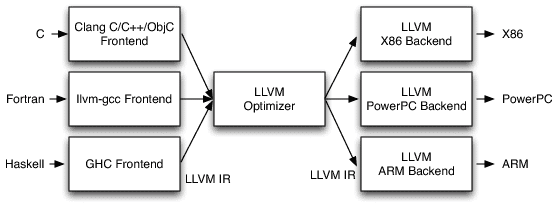
\includegraphics{llvm}
\caption{Overview of LLVM Architecture.}
\label{fig:llvm}
\end{center}
\end{figure}

For a \textit{runtime} compiler, the back end is modified to provide for emitting, loading, relocating, and linking native machine language at run time. The LLVM/Clang system that does this is called the on-request compiler (ORC) \citep{llvmorc}. It is a type of just-in-time (JIT) compiler that emits native machine language for a symbol the very first time  the address of that symbol is requested from the LLVM execution session. The ORC compiler and LLVM can load and link external dynamic link libraries --- whether system libraries, or user libraries, or LLVM's own in-memory JITDylib libraries -- at run time, and thus perform the functions of a build system linker or an operating system's linking loader.

% How the opcodes work

As an example of how to embed a runtime C++ compiler into a SWSS, we present two new opcodes for Csound: \texttt{clang\_compile} and \texttt{clang\_invoke}. These opcodes are available on GitHub \cite{clangopcodes}, and are documented there. 





% How to use the opcodes

% format for Heading-B style
\subsection{Format for Heading-B Style}

Insert body text here.  
Use the Heading-B style for headings of subsections.

% format for Heading-C style
\subsubsection{Format for Heading-C Style}

Insert body text here.
Use the Heading-C style for headings of sub-subsections.

In the initial manuscript submission, you are encouraged to include figures (with captions) inline with the text, for ease of reading during the review process. 
All figures will need to be grayscale (i.e.,~monochrome) and sufficiently high-resolution for print (300 dpi), at the latest by your final submission.
Figures must be referenced in the text, either directly in the text or as a parenthetic aside, e.g.~``(see Figure~\ref{fig:myFigure}).''
Do not reference figures with terms of relative location like ``above'' or ``below,'' however.
When an article is typeset, figures are never embedded in the text and you do not know exactly where the image will appear in relation to your text.
For the review process, simply place the LaTeX figure definition immediately after the first paragraph referring to the image.

% include figures in text with captions for initial submission, like this:
\begin{figure}[]
\begin{center}
\includegraphics{myFigure}
	% No need for file extensions here! 
	% This is useful at final submission, when MIT Press and LaTeX need different image formats for the same image
	% This template is already set up to look for image files in the Figures subdirectory, so that's where to put your image files. 
\caption{Insert Figure caption here.}
\label{fig:myFigure}
\end{center}
\end{figure}

Tables must also be cited in the text, as with Table~\ref{tab:myTable}. Tables in \emph{CMJ} do not have ``captions'' as such. A table has a title, which should be concise. If absolutely necessary for understanding the table, additional information can be included in a footer, although that is not required. When typeset, tables will not have vertical rules.

% include tables in text with captions for initial submission, like this:
\begin{table}[]
\caption{Sample Table with a Title}
\centering
\begin{tabular}{lccr}
  \hline
  \textbf{Column} & \textbf{Headers} & \textbf{Might Look} & \textbf{Like This}  \\
  \hline
  one & 2 & 3 & IV \\
  five & 6 & 7 & VIII \\
  nine & 10 & 11 & XII \\
   \hline
\end{tabular}
\caption*{\textnormal{{\small Although table footers are often not necessary, the source code shows how to generate one using an unnumbered caption in LaTeX.}}}
\label{tab:myTable}
\end{table}%


For the final version after the manuscript has been accepted, however, all figures and tables should be moved to the end.
The recommended way to achieve this is by enabling the package {\tt endfloat} as noted in the comments at the of top the LaTeX template file.

Also note that for the final version of your article, MIT Press requires grayscale versions of your artwork in either EPS (vector image) or TIFF (raster) formats.
In general, LaTeX only supports PDF, PNG, and JPEG formats for images.
The upshot of this is that authors using LaTeX need to submit images in two formats.
The good news is that most LaTeX implementations provide utilities for converting from the formats used by MIT Press to those used by LaTex.

% equations
You can insert equations inline with the text like this:

\begin{equation}
	\label{radupdate}
		\Psi_{N}^{n+1} = m_{N}^{(-)}\Psi_{N-1}^{n}+m_{N}^{(0)}\Psi_{N}^{n} + q_{N}\Psi_{N}^{n-1}
\end{equation}
where
\begin{eqnarray*}
	m_{N}^{(-)} &=& \frac{\lambda^2}{2\tau}\left(S_{N+1}+2S_{N}+S_{N-1}\right)\\
	m_{N}^{(0)} &=& \frac{1}{\tau}\left(2-\frac{\lambda^2}{2}\left(S_{N+1}+2S_{N}+S_{N-1}\right)\right)\\
	q_{N} &=& \frac{1}{\tau}\left(\frac{\gamma^2 k^2}{2h}\left(S_{N+1}+S_{N}\right)\left(\frac{\alpha_{1}}{k}-	\alpha_{2}\right)-1\right)
\end{eqnarray*}
and where 
\begin{equation*}
	\tau = \frac{\gamma^2 k^2}{2h}\left(S_{N+1}+S_{N}\right)\left(\frac{\alpha_{1}}{k}+\alpha_{2}\right)+1
\end{equation*}

% Use this environment for inserting source code examples.
% Note, that this will print out text in the document exactly as you type it here in the .tex file. That means you can add empty spaces, tabs, blank lines here and they will be printed out like this in the document.). 
%For more information check out the LaTeX-Package 'fancyvbr' documentation
%
\begin{Verbatim}[fontfamily=courier, xleftmargin=\parindent]
Use this style for program code, 
for example:
main() {
    printf("Hello World\n");    
}
Extended code examples that are likely
to be too wide for the two-column page
layout used by CMJ should be prepared
as figures, using text rather than an
image format. You don't need to worry
about this for the initial submission, 
but it will become important after 
acceptance for the final submission.
\end{Verbatim}

%use of references
Some examples for the use of references in the text follow.
%author name in sentence, single authors
Single authors, listed separately in text: for instance, \citet*{Ano08} or \citet*{Bele68}.
%author name in sentence, multiple authors
Multiple authors, in text: \citet*{VeRo00}; \citet*{AtDa04}.
Parenthetic citations: \citep*{AtDa04, Ther99}.
Citation as a single parenthetic note, including supplementary information, \citep*[see also][which includes detailed diagrams]{Zica02}.
Please don't type parentheses around a \texttt{citet*{}} directive when you want a citation in parentheses---that's what the \texttt{citep*{}} family of directives are there for.
And it is preferable to use the starred versions of BibTeX directives (\texttt{citet*\{\}} rather than \texttt{citet\{\}}, etc.)

Please consult the enclosed .bst file and the BibTeX documentation for further examples. 


%References
\bibliographystyle{cmj}
\bibliography{EmbeddingClangLLVMinCsound}

\end{document}
